\chapter{Phenotype Control of Partially Specified Boolean Networks}
\label{chapter:phenotype_control_psbn}

% \begin{enumerate}
%     \item CMSB2023
%     \item What? why?
%     \item Robustness
%     \item Algorithm
%     \item Example
%     \item Performance/scalability
% \end{enumerate}


Finally, we can discuss the topic of phenotype control for PSBNs: we assume a set of phenotype states $P \subseteq \bools^n$ and the goal is to perturb the network such that it \emph{exhibits} this phenotype. In other words, after the perturbation is applied to the network, the network stabilizes in some attractor $A$ such that $A \subseteq P$. However, in the presence of partially unknown dynamics, this may not be achievable using a sufficiently small perturbation. In such cases, we rely on control \emph{robustness} to assess viability of possible perturbations.

\section{Problem Definition}
\label{s:phenotype_problem_definition}

As before, for simplicity, we first introduce some of the concepts for classical BNs and then expand these to PSBNs. First, to control the behaviour of a BN, we use the notion of variable perturbation:

\begin{definition}
	A \emph{variable perturbation} is a vector $Q \in \bools_\unspecified^n$. For every $Q_i = {\unspecified}$, we say that the $i$-th variable is \emph{unperturbed}, whereas for $Q_i = 0$ or $Q_i = 1$, we say the variable is \emph{perturbed} to either $0$ or $1$.
\end{definition}

We write $\mathit{fixed}(Q)$ and $\mathit{free}(Q)$ to denote the subset of perturbed and unperturbed variables, respectively. The \emph{size} of $Q$ is the size of the $\textit{fixed}(Q)$ set. Furthermore, a perturbation can again be seen as a \emph{subspace} of $\bools^n$. We then write that the states in this subspace are \emph{compliant} with $Q$.

For a particular $\mathbb{BN}$ and $Q$, we consider a \emph{perturbed} state-transition graph $\STG[Q](\mathbb{BN})$, which is a sub-graph of $\STG(\mathbb{BN})$ \emph{induced} by the states compliant with $Q$. Intuitively, the $\mathit{fixed}(Q)$ variables are restricted to their perturbed values, while $\mathit{free}(Q)$ variables are left to evolve without modification. 

%\begin{definition}
We say that a~permanent variable perturbation $Q \in \bools_\unspecified^n$ \emph{controls} Boolean network $\mathbb{BN}$ towards phenotype $P$ if and only if $\mathcal{A}(\STG[Q](\mathbb{BN})) \subseteq P$.
%\end{definition}
Intuitively, a perturbation represents an effective control strategy if it causes the network to only exhibit attractors from the desired phenotype $P$. However, note that $\mathcal{A}(\STG[Q](\mathbb{BN}))$ is not necessarily a subset of $\mathcal{A}(\STG(\mathbb{BN}))$. A permanent perturbation can disturb existing attractors or even introduce new ones.

This concept naturally applies to interpretations of PSBNs as well: given a $\mathbb{PSBN}$, an interpretation $\mathcal{I}$ and a perturbation $Q$, the interpretation has a perturbed $\STG[Q](\mathbb{PSBN}(\mathcal{I}))$. As such, a perturbation $Q$ controls $\mathbb{PSBN}$ under the interpretation $\mathcal{I}$ if it ensures $\mathcal{A}(\STG[Q](\mathbb{PSBN}(\mathcal{I}))) \subseteq P$.

\begin{example}
	Consider the network from \autoref{example:psbn}, a phenotype $P = 1 \unspecified \unspecified$ and a perturbation $Q = \unspecified 1  \unspecified$. \autoref{subfig:perturbed_stg} depicts the perturbed STGs of interpretations $\mathcal{I}_{0101}$ and $\mathcal{I}_{0110}$, with phenotype states highlighted in green. Perturbation $Q = \unspecified 1  \unspecified$ achieves control for interpretation $\mathcal{I}_{0101}$, but not for $\mathcal{I}_{0110}$.
\end{example}

\begin{definition}
	Assume a partially specified network $\mathbb{PSBN}$, a phenotype $P \subseteq \bools^n$ and a set of admissible perturbations $\mathcal{Q} \subseteq \bools_\unspecified^n$. The goal of the \emph{complete} phenotype control is to compute all pairs $(c, Q) \in \bools^m \times \bools_\unspecified^n$ such that $Q \in \mathcal{Q}$ and $Q$ controls $\mathbb{PSBN}(\mathcal{I}_c)$ towards phenotype $P$.
\end{definition}

Intuitively, the result of PSBN phenotype control are all combinations of colours and perturbations for which the perturbation necessarily stabilizes the associated network interpretation in the given phenotype. The set $\mathcal{Q}$ is in practice used to restrict the problem setting to perturbations of a certain size or to otherwise biologically feasible perturbations.

\paragraph{Perturbation size and robustness}

In practice, it is often unnecessary to compute the complete set of colour-perturbation pairs. The goal is instead to find the smallest functioning perturbation~\cite{Su2019CMSB,Su2020}. However, in partially specified networks, such minimal perturbation typically only works for a small subset of interpretations, making it potentially unreliable in practice. To address this, we consider robust phenotype control:

\begin{definition}
	The \emph{robustness} $\rho$ of a perturbation $Q \in \bools_\unspecified^n$ is defined as:
	\begin{align*}
		\rho(Q) = \frac{|\{ c \in \bools^{m} \mid Q~\text{\upshape controls}~\mathbb{PSBN}(\mathcal{I}_c) \}|}{|\bools^{m}|}
	\end{align*}
	Given a robustness threshold $r \in (0,1]$, the goal of \emph{robust} phenotype control is to compute the smallest perturbation (or perturbations) $Q$ s.t. $\rho(Q) \geq r$.
\end{definition}

Ideally, a suitable perturbation $Q$ with $\rho(Q) = 1$ achieves control for all interpretations of $\mathbb{PSBN}$. However, if no such perturbation exists, the parameter $r$ can be tuned to achieve a trade off between perturbation size and robustness.

\section{Methods}
\label{sec:Methods}

%TODO: Vyzdvihnut, co je rovnake z Biosystems2023

Partially specified Boolean networks suffer from both state and parameter space explosion, which in practice makes them hard to analyse exhaustively. In the context of control, this problem is further complicated by perturbation space explosion. To mitigate this, we employ symbolic state space exploration which allows us to analyse the full set of possible perturbed STGs within a single algorithm pass. This technique exploits similarities between the STGs of various network interpretations (and perturbations) to significantly speed up the exploration process compared to the naive enumeration~\cite{aeonpy,Brim2021}.

\subsection{Symbolic computation model}

A binary decision diagram (BDD)~\cite{Bryant86} is a directed acyclic graph which represents a Boolean function. A BDD-encoded function $f: \bools^k \to \bools$ can be used to encode a set (or relation) of Boolean vectors $X \subseteq \bools^k$, such that $f(x) = 1 \Leftrightarrow x \in X$. Since both network states ($\bools^n$) and interpretations ($\bools^m$ after normalisation) correspond to Boolean vectors, such sets have a direct BDD representation.

For sets of perturbations, a naive approach requires two Boolean variables per component, since their domain is $\bools_\unspecified$ instead of $\bools$. However, in~\cite{brim2022}, we introduce an alternative encoding suitable for representing perturbed state-transition systems that only requires one variable. This significantly improves the efficiency of the encoding, since fewer symbolic variables typically result in smaller BDDs.

\paragraph{Perturbed STG encoding} Observe that in the context of a state $x \in \bools^n$ which is \emph{compliant} with a perturbation $Q$, it is sufficient to know the set $\mathit{fixed}(Q)$ to fully reconstruct $Q$: we have $Q_i = x_i$ for every $i \in \mathit{fixed}(Q)$ and $Q_i = \unspecified$ otherwise. 

Consequently, a relation over states $x$, interpretations $\mathcal{I}_c$ and perturbations $Q$ where all states are compliant with their respective perturbations can be encoded as a relation over $\bools^n \times \bools^m \times \bools^n$. Here, the last component encodes the possible sets $\mathit{fixed}(Q)$. Since each perturbed $\STG[Q](\mathbb{BN})$ only admits states compliant with $Q$, such representation is suitable for collectively encoding dynamics of such perturbed STGs for different perturbations. 

To avoid confusion, we write $\mathcal{V} \equiv \bools^n$ to mean the set of network states, $\mathcal{C} \equiv \bools^m$ to mean the set of network interpretations (colours), and $\mathcal{L} \equiv \bools^n$ to mean the set of sets of perturbed variables $\mathit{fixed}(Q)$, collectively $\mathcal{S} = \mathcal{V} \times \mathcal{C} \times \mathcal{L}$. For $(x,l) \in \mathcal{V} \times \mathcal{L}$, we also write that $Q \equiv (x,l)$ when $Q_i = x_i$ for all $l_i = 1$ and $Q_i = \unspecified$ when $l_i = 0$ (i.e. $Q$ can be reconstructed based on the state $x$ and the set of perturbed variables $l$). 

When the goal is to symbolically represent a subset of perturbations $\mathcal{Q} \subseteq \bools_\unspecified^n$, we do this through a relation $S_{\mathcal{Q}} \subseteq \mathcal{V} \times \mathcal{L}$ where $S_{\mathcal{Q}}$ contains exactly \emph{all} states compliant with every $Q \in S$. Finally, in some cases, we may need to directly reference the Boolean BDD variables used in our encoding. We then use the notation $\mathcal{V}_i$, $\mathcal{C}_i$, resp. $\mathcal{L}_i$ to denote the $i$-th BDD variable that encodes the state, colour or perturbation component of $\mathcal{S}$.

\paragraph{Symbolic operations} Set operations ($\cap, \cup, \setminus$, etc.) on symbolic sets (or relations) are implemented through Boolean logical operators ($\land, \lor, \neg$, etc.) as is customary for BDDs. Furthermore, the following standard BDD operations are used:
\begin{align*}
	\textsc{Project}_{\mathcal{X}}(X \subseteq \mathbb{B}^k)&= \{ x \in \mathbb{B}^k \mid \exists b \in \bools.~x[\mathcal{X} \mapsto b] \in X \}\\
	\textsc{Select}_{\mathcal{X}=b}(X \subseteq \mathbb{B}^k)&= \{ x \in \mathbb{B}^k \mid x \in X \land x[\mathcal{X}] = b \}\\	
	\textsc{Restrict}_{\mathcal{X}=b}(X \subseteq \mathbb{B}^k)&=\textsc{Project}_{\mathcal{X}}(\textsc{Select}_{\mathcal{X}=b}(X))
\end{align*}

Here, $\mathcal{X}$ denotes a variable of the BDD encoding (e.g. $\mathcal{V}_3$). We can also use a list of conditions in the subscript of the method as a shorthand for multiple nested calls to the same method. Intuitively, $\textsc{Project}$ is equivalent to existential quantification, $\textsc{Select}$ is implemented through conjunction, and $\textsc{Restrict}$ is a combination of both. To explore the perturbed STGs, we use:
\begin{align*}
      \pre(X \subseteq \mathcal{S}) &= \{~(s, c, l) \mid \exists (t, c, l) \in X.~s \to_{c,Q}^{} t \text{ for } Q \equiv (s, l)~\}\\
      \post(X \subseteq \mathcal{S}) &= \{~(t, c, l) \mid \exists (s, c, l) \in X.~s \to_{c,Q}^{} t \text{ for } Q \equiv (s, l)~\}
\end{align*}
Here, $s \to_{c,Q} t$ denotes that $s \to t$ within the graph $\STG[Q](\mathbb{PSBN}(\mathcal{I}_c))$. Intuitively, $\pre$ and $\post$ compute the sets of predecessors and successors of the states in $X$ within $\mathbb{PSBN}$ under their respective interpretations $\mathcal{I}_c$ and perturbations $Q$. The implementation details of these operations can be found in~\cite{brim2022}.

We then rely on a method $\textsc{Trap}(X \subseteq \mathcal{S})$ which computes the \emph{maximal trap set} within the given set $X$. Naively, this method can be implemented as the greatest fixed point of $\textsc{Trap}(X) = X \cap \textsc{Trap}(X \setminus \textsc{Pre}(\textsc{Post}(X)))$. However, we use a more efficient implementation based on the technique called \emph{saturation}~\cite{benevs2022bdd}.

Finally, we use $\mathbb{VAL}_k^n$ to denote a BDD which encodes a function of $n$ inputs that is $\mathit{true}$ iff exactly $k$ inputs are $\mathit{true}$. To construct such BDD efficiently, we observe that $\mathbb{VAL}_0^n = \bigwedge_{i \in [1,n]} \neg x_i$, and that $\mathbb{VAL}_k^n = \bigvee_{i \in [1,n]} (\mathbb{VAL}_{k-1}^n \lor x_i)$.

\subsection{Control algorithm}

Our control approach is based on \autoref{algo:control} where we describe:

\begin{itemize}
	\item $\textsc{CompletePhenotypeControl}$: Core algorithm that iteratively computes the \emph{complete} control map for an admissible set $\mathcal{Q}$.
	\item $\textsc{RobustPhenotypeControl}$: A wrapper for the core algorithm that facilitates minimal control under the desired \emph{robustness}.
	\item $\textsc{Enumerate}$: An auxiliary method to enumerate all \emph{working} perturbations and find the maximum robustness.
\end{itemize}


\begin{algorithm}[ht!]
  \SetKwProg{Fn}{Fn}{}{}
	\Fn{\upshape \textsc{CompletePhenotypeControl}$(P \subseteq \mathcal{V}, \mathcal{Q} \subseteq \mathcal{V} \times \mathcal{L} ~(\text{encodes~}\bools_\unspecified^n))$}{
		$\var{universe} \gets \{~(x, c, l) \in \mathcal{S} \mid (x,l) \in \mathcal{Q}~\}$\;
		$\var{phenotype} \gets \var{universe} \cap (P \times \mathcal{C} \times \mathcal{L})$\;
		$\var{phenotype\_trap} \gets \textsc{Trap}(\var{phenotype})$\;
		$\var{non\_phenotype} \gets \var{universe} \setminus \var{phenotype\_trap}$\;
		$\var{cannot\_control} \gets \textsc{Trap}(\var{non\_phenotype})$\;
		\For{$i \in [1,n]$}{
			$\var{not\_perturbed} \gets \textsc{Project}_{\mathcal{V}_i}(\textsc{Select}_{\mathcal{L}_i = 0}(\var{cannot\_control}))$\;
			$\var{cannot\_control} \gets \var{not\_perturbed} \cup \textsc{Select}_{\mathcal{L}_i = 1}(\var{cannot\_control})$\;
		}
		$\var{control\_map} \gets \var{universe} \setminus \var{cannot\_control}$\;
		\Return{\upshape$\var{control\_map}$}\;
	}
	\Fn{\upshape \textsc{RobustPhenotypeControl}$(r, P \subseteq \mathcal{V}, \mathcal{Q} \subseteq \mathcal{V} \times \mathcal{L})$}{
		\For{$k \in [0,n]$}{
			$\mathcal{Q}_k \gets \mathcal{Q} \cap (\mathcal{V} \times \mathbb{VAL}_k^n)$\;
			$\var{control\_map} \gets \textsc{CompletePhenotypeControl}(P, \mathcal{Q}_k)$\;
			$\rho_{\var{best}}  \gets \textsc{Enumerate}(1, \var{control\_map})$\;
			\lIf{$\rho_{\var{best}} \geq r$}{\Return{}}
		}
	}
	\Fn{\upshape \textsc{Enumerate}$(i \in \mathbb{N}, \var{control\_map} \subseteq \mathcal{S}~(\text{encodes}~\bools^m \times \bools^n_\unspecified))$}{
		\lIf{\upshape$\var{control\_map} = \emptyset$}{\Return{$0$}}
		\lIf{$i > n$}{\Return{\upshape$\frac{|\{c \in \mathcal{C}\mid\exists (x,c,l) \in \mathcal{S}. (x, c, l) \in \var{control\_map}\}|}{|\mathcal{C}|}$}}
		$\var{not\_controlled} \gets \textsc{Restrict}_{\mathcal{L}_i = 0}(\var{control\_map})$\;
		$\var{controlled\_true} \gets \textsc{Restrict}_{\mathcal{L}_i = 1, \mathcal{V}_i = 1}(\var{control\_map})$\;
		$\var{controlled\_false} \gets \textsc{Restrict}_{\mathcal{L}_i = 1, \mathcal{V}_i = 0}(\var{control\_map})$\;
		$\var{best} \gets \textsc{Enumerate}(i+1, \var{not\_controlled})$\;
		$\var{best} \gets \mathit{max}(\var{best}, \textsc{Enumerate}(i+1, \var{controlled\_true}))$\;
		$\var{best} \gets \mathit{max}(\var{best}, \textsc{Enumerate}(i+1, \var{controlled\_false}))$\;		
		\Return{\upshape\var{best}}\;
	}
	\caption{Symbolic permanent phenotype control of PSBNs.}
	\label{algo:control}
\end{algorithm}

\paragraph{Complete control} The main idea behind \autoref{algo:control} is the following: A perturbation achieves phenotype control if and only if all attractors in the perturbed STG are within the phenotype subset $P$. Consequently, we want to \emph{discard} any perturbation that provably retains some attractor not contained in $P$. 

% A possible way of doing this would be to compute all attractors of the system under admissible perturbations and then discard perturbations where non-phenotype attractor state is detected. However, this approach can be problematic if the number of distinct attractors in different perturbations is too large.

% Instead, we compute a larger non-phenotype trap set that is guaranteed to contain all non-phenotype attractor states in it. To do so, we first compute a similar trap subset of the phenotype $P$ which is guaranteed to contain all phenotype attractors. Then, we invert this set and repeat the operation to obtain a trap which is a superset of all non-phenotype attractors.

Therefore, we compute a non-phenotype trap set that is guaranteed to contain all non-phenotype attractor states in it. First, we compute a similar trap subset of the phenotype $P$ which is guaranteed to contain all phenotype attractors. Then, we invert this set and repeat the operation to obtain a trap which is a superset of all non-phenotype attractors. Note that simply computing the largest trap set within $\mathcal{V} \setminus P$ would only cover attractors that are completely within $\mathcal{V} \setminus P$. The above-described process is necessary to also cover attractors that intersect $P$ but are not subsets of $P$.

The algorithm then iterates over all network variables and performs projection in cases where the variable is \emph{not perturbed}. Initially, the \var{cannot\_control} set contains at least one state of the perturbed STG of each $Q \in \mathcal{Q}$ that admits a non-phenotype attractor. After this operation, \var{cannot\_control} contains \emph{all} states of such perturbed STG. In other words: the resulting set can depend on variable $\mathcal{V}_i$ only if $\mathcal{L}_i = 1$ (i.e. the variable is perturbed). In such cases, the role of $\mathcal{V}_i$ is to encode the actual perturbed value of the $i$-th network variable. 

Finally, we invert the \var{cannot\_control} set to only retain perturbations where no non-phenotype attractor state exists.

\paragraph{Robust control}

To extend this algorithm to robust control, we test the perturbations of increasing size (using the $\mathbb{VAL}_{k}^{n}$ BDD) and use a recursive $\textsc{Enumerate}$ method to find perturbations with maximal robustness. Notice that the necessity of this step makes our algorithm \emph{semi-symbolic}. 

Instead of iterating through all possible control strategies of size $k$, procedure $\textsc{Enumerate}$ recursively branches into three cases for each variable $i$: $i$ is not perturbed, $i$ is perturbed to $\mathit{true}$, and $i$ is perturbed to $\mathit{false}$. Note that each call completely eliminates both $\mathcal{L}_i$ and $\mathcal{V}_i$ from \var{control\_map} (for the case of $\mathcal{L}_i = 0$, $\mathcal{V}_i$ was already eliminated by the core algorithm). As such, once $i > n$, the resulting \var{control\_map} only depends on variables $\mathcal{C}_i$ and we can use it to compute the robustness.

Note that for simplicity, we do not store the actual perturbations with maximal robustness explicitly in the algorithm. However, these can be easily reconstructed from the recursion path in the \textsc{Enumerate} algorithm. Furthermore, note that the recursion in the \textsc{Enumerate} algorithm can be replaced using \emph{projected iteration}, where we first project the \var{control\_map} to the admissible $l \in \mathcal{L}$, and then project only to the state variables perturbed within each such $l$. This approach can be faster as it uses fewer symbolic steps. However, it is also highly specific to each BDD library. As such, we chose to present the more widely applicable algorithm.


\begin{algorithm}[ht!]
	\SetKwProg{Fn}{Fn}{}{}
	  \Fn{\upshape \textsc{IsPhenotypeControlAux}$(\phenotype \subseteq \vertices, \var{osc\_allowed} \in \bools, \var{init\_states} \subseteq \vertices$}{
	  $\var{phenotype\_space} \gets$ \leIf{\upshape $\var{osc\_allowed}$}{$ \textsc{Bwd}(\phenotype)$}{\phenotype}
	  $\var{phenotype\_trap} \gets \textsc{Trap}(\phenotype)$\;
	  $\var{reachable} \gets \textsc{Fwd}(\var{init\_states})$\;
		  $\var{non\_phenotype} \gets \, \var{reachable} \setminus \var{phenotype\_trap}$\;
	  $\var{non\_phenotype\_trap} \gets \textsc{Trap}(\var{non\_phenotype})$\;
		  \Return{\upshape \leIf{$\var{non\_phenotype\_trap} = \emptyset$}{true}{false}}
	  }
	  \Fn{\upshape \textsc{IsPhenotypeControl}$(\phenotype \subseteq \vertices, \var{phen\_type} \in \{ stabilize, avoid, oscillate\}, \var{init\_states} \subseteq \vertices)$}{
	  \uIf{\upshape $\var{phen\_type} = stabilize$}{
		\Return{\textsc{IsPhenotypeControlAux}($\phenotype, false, \var{init\_states}$)}\;
	  }
	  \uElseIf{\upshape $\var{phen\_type} = avoid$}{
		$\phenotype' \gets \vertices \setminus \phenotype$\;
		\Return{\textsc{PhenotypeControlAux}($\phenotype', false, \var{init\_states}$)}\;
	  }
	  \uElseIf{\upshape $\var{phen\_type} = oscillate$}{
		$\phenotype' \gets \vertices \setminus \phenotype$\;
		$\var{in\_phen} \gets \textsc{PhenotypeControlAux}(\phenotype, true, \var{init\_states})$\;
		$\var{out\_phen} \gets \textsc{PhenotypeControlAux}(\phenotype', true, \var{init\_states})$\;
		\Return{\upshape$\var{in\_phen} \land \var{out\_phen}$}\;
	  }
	}
	  \caption{Phenotype verification algorithms}
	  \label{algo:control}
  \end{algorithm}
  
  Since we encode all network instances and perturbation variants into a single graph, our algorithm aims to verify whether the given network is fulfilling the control objective (i.e. the whole network has the given relationship toward the phenotype) or not. The main method for that is shown in \autoref{algo:control}. 
  
  Even though there are three types of relationships between a network and a phenotype, the core of our algorithm \textsc{IsPhenotypeControlAux} relies on two different relationships -- we see the oscillation as either allowed or forbidden. 
  
  
  \begin{figure}[ht!]
	\subfloat[BN not stabilizing in phenotype $\phenotype$ due to the non-phenotype attractor.]{
	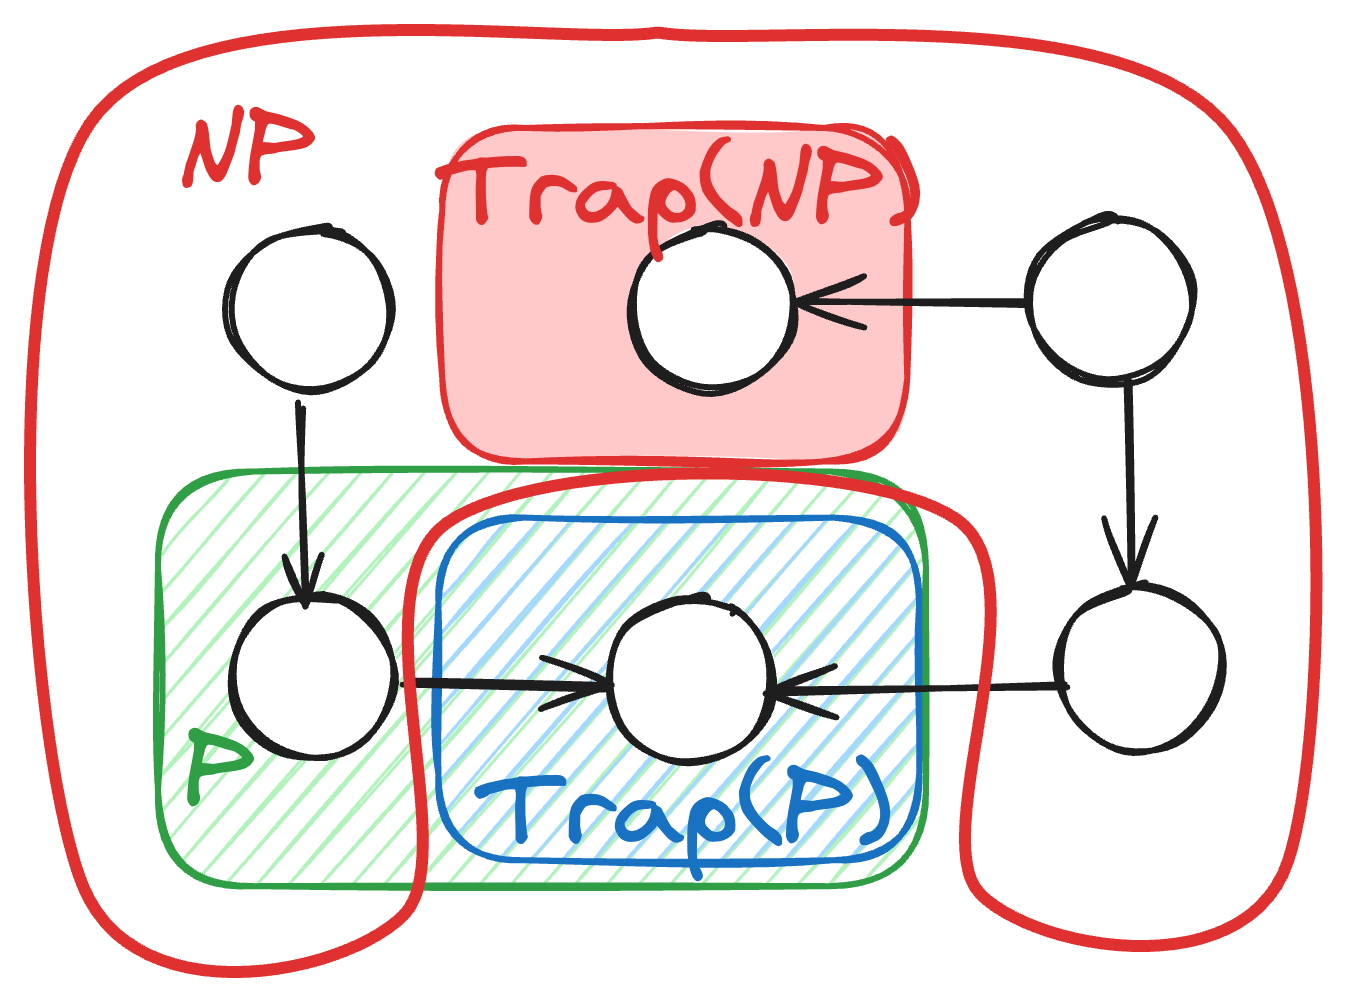
\includegraphics[width=0.45\textwidth]{Figures/algo_exp_a.png}
	\label{subfig:algo_a}
	}
	\hspace*{10pt}
	\subfloat[BN not stabilizing in phenotype $\phenotype$ due to the oscillating phenotype attractor.]{
	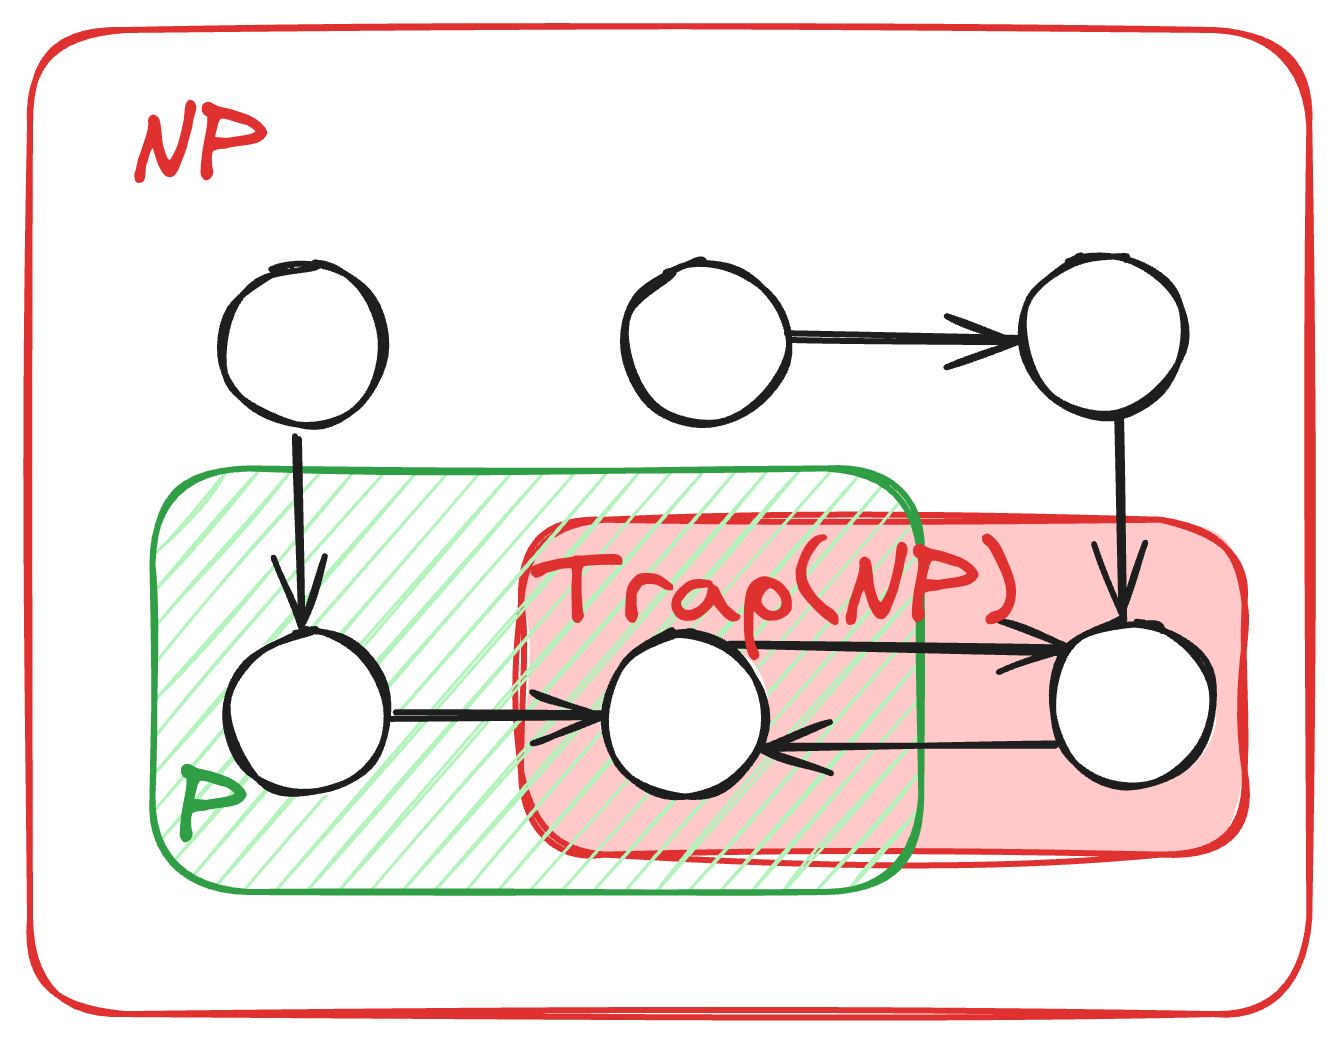
\includegraphics[width=0.45\textwidth]{Figures/algo_exp_b.png}
	\label{subfig:algo_b}
	} \newline
	\subfloat[BN exhibiting oscillating phenotype $\phenotype$ -- computation of $\phenotype$.]{
	\centering
	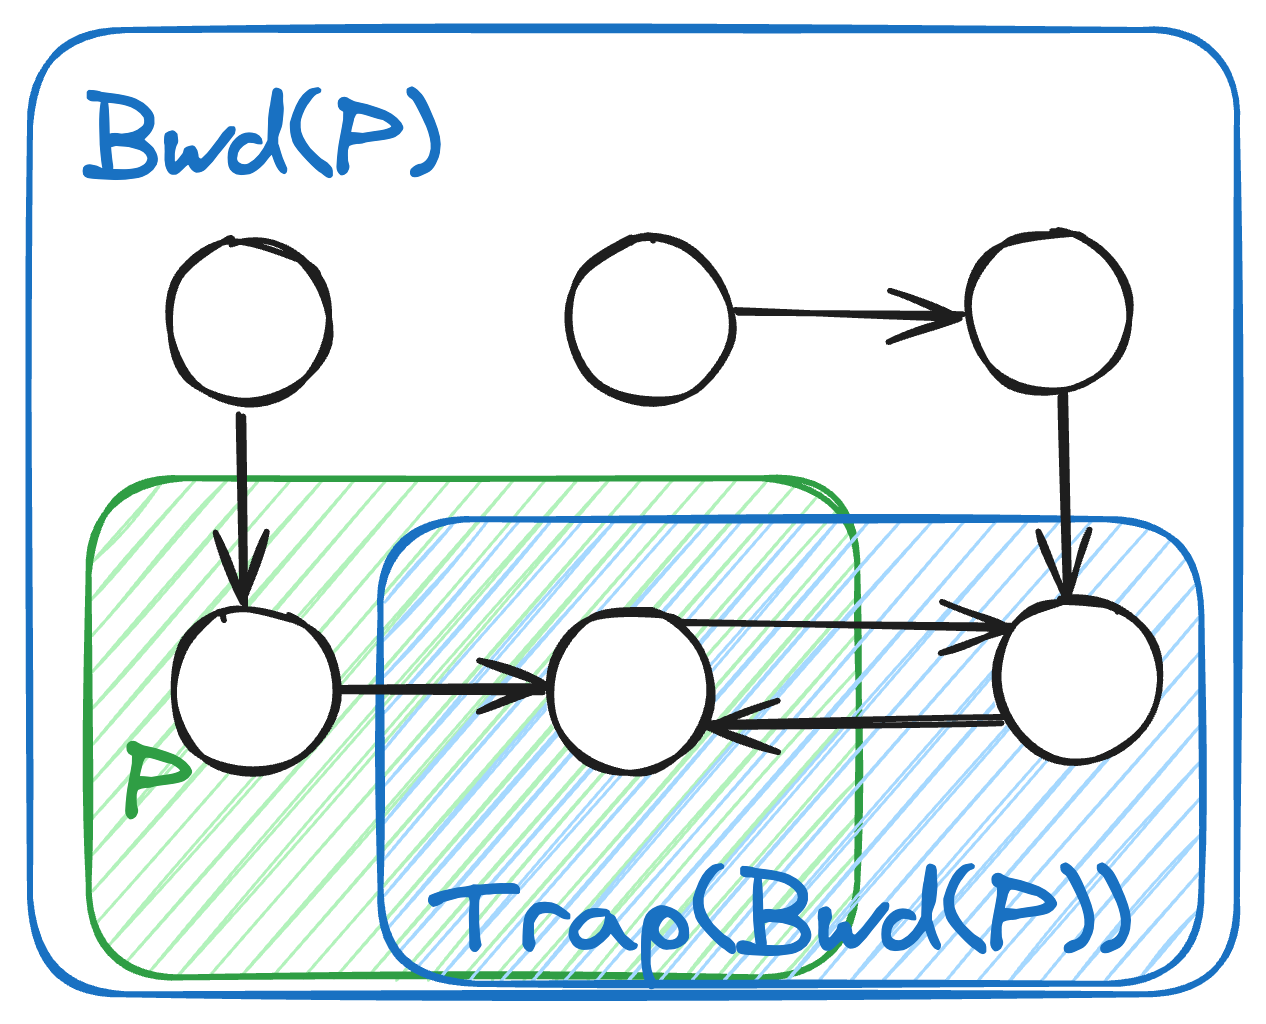
\includegraphics[width=0.45\textwidth]{Figures/algo_exp_c.png}
	\label{subfig:algo_c}
	}
	\hspace*{10pt}
	\subfloat[BN exhibiting oscillating phenotype $\phenotype$ -- computation of $\phenotype' = \vertices \setminus \phenotype$.]{
	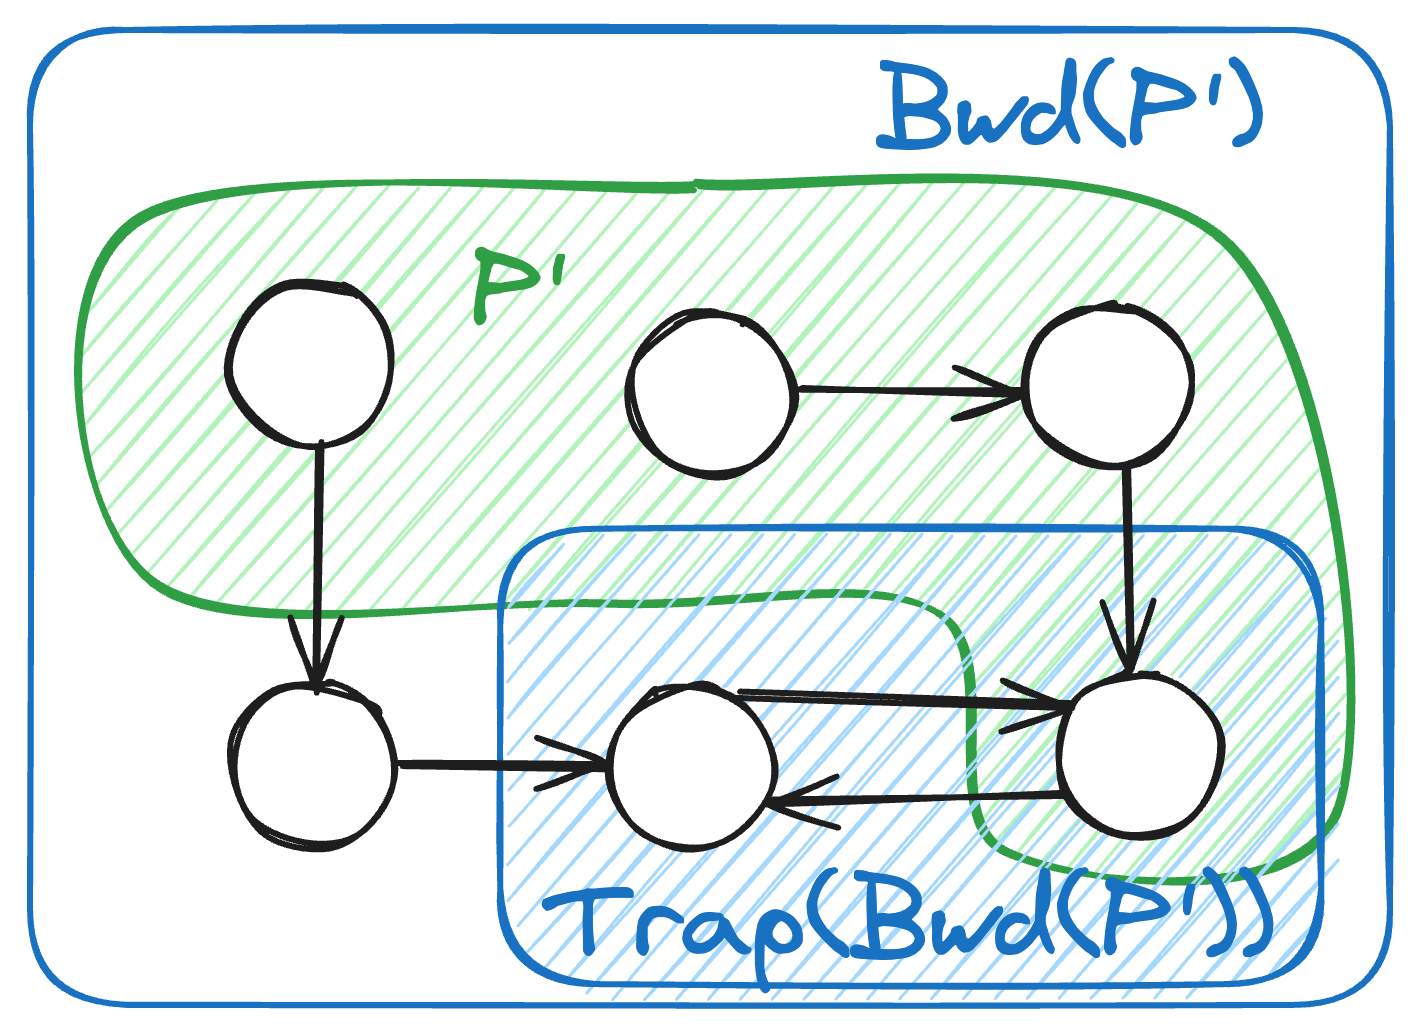
\includegraphics[width=0.45\textwidth]{Figures/algo_exp_d.png}
	\label{subfig:algo_d}
	} \newline
	\subfloat[BN not exhibiting oscillating \phenotype $\phenotype$ -- computation of $\phenotype$.]{
	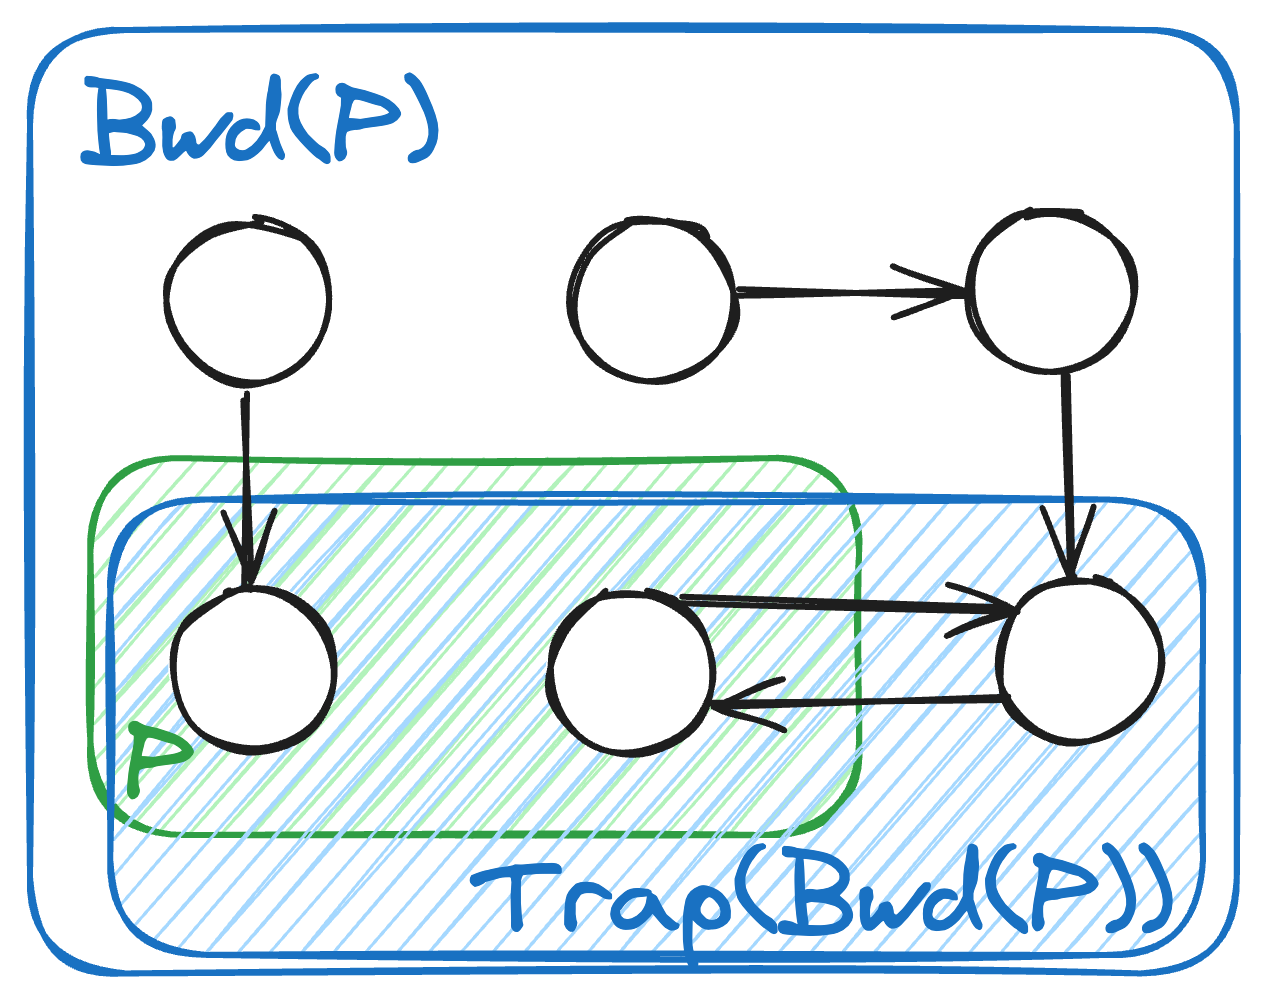
\includegraphics[width=0.45\textwidth]{Figures/algo_exp_e.png}
	\label{subfig:algo_e}
	}
	\hspace*{10pt}
	\subfloat[BN not exhibiting oscillating phenotype $\phenotype$ -- computation of $\phenotype' = \vertices \setminus \phenotype$.]{
	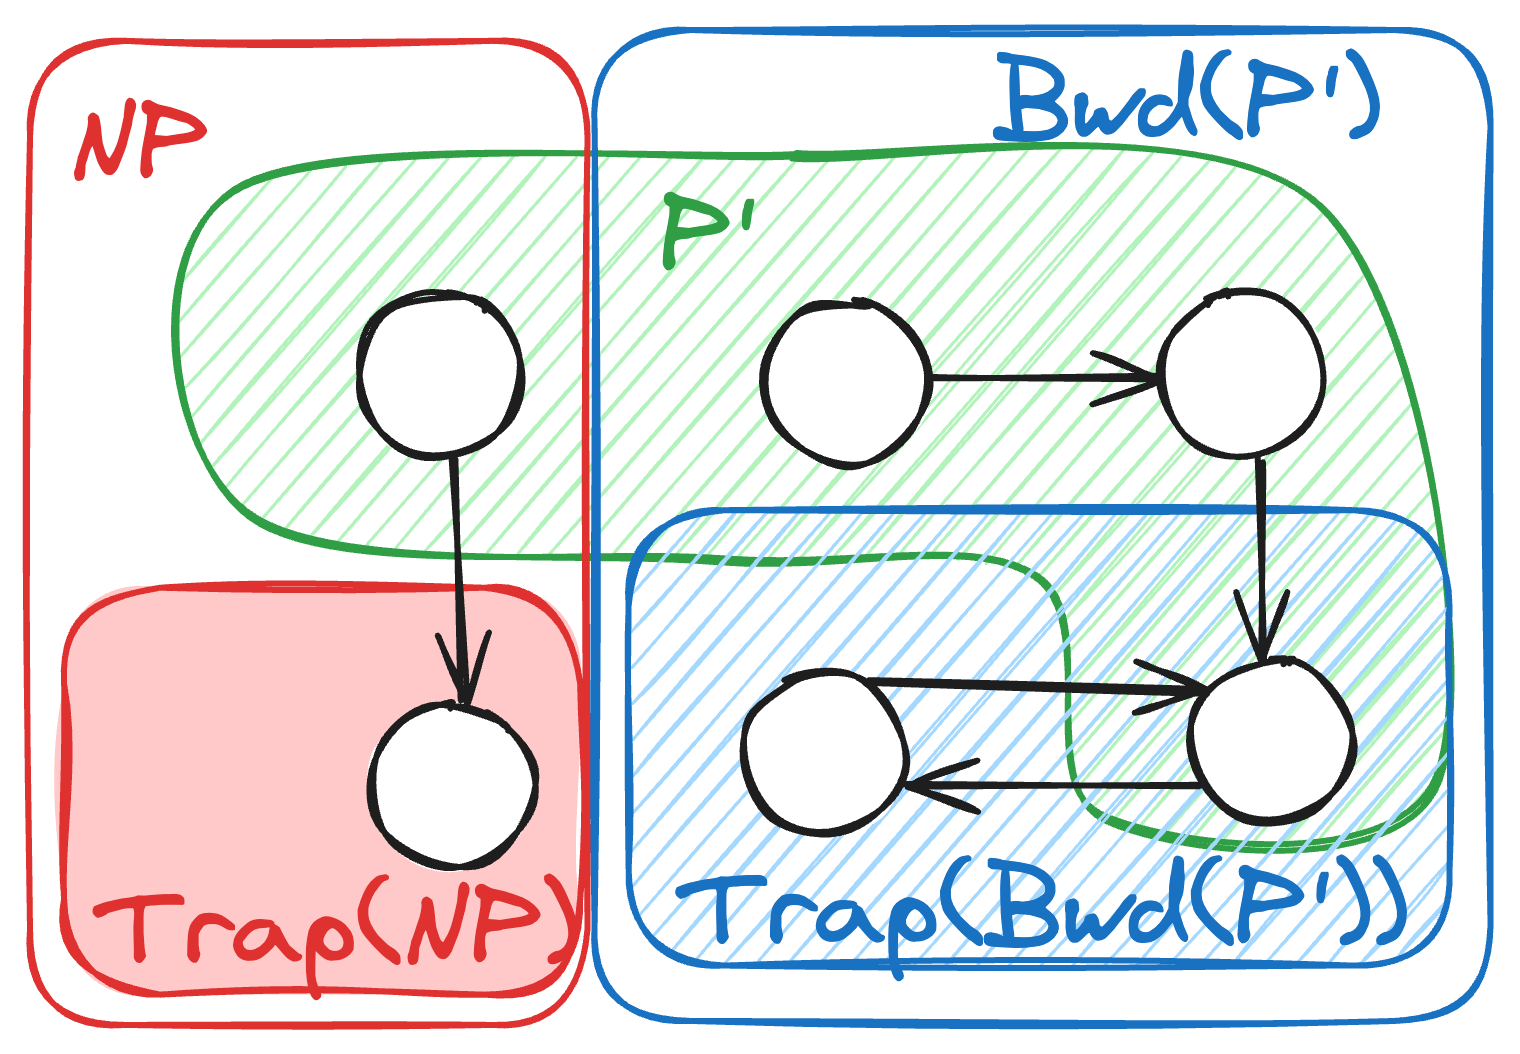
\includegraphics[width=0.45\textwidth]{Figures/algo_exp_f.png}
	\label{subfig:algo_f}
    }
	\caption{\textbf{Examples of \autoref{algo:control} progressions.} \autoref{sub@subfig:algo_a} and \autoref{sub@subfig:algo_b} show situations where BN does not stabilize in the given phenotype considering not allowed oscillation. \autoref{sub@subfig:algo_c} and \autoref{sub@subfig:algo_d} show the computation of the oscillating phenotype $\phenotype$ and its complement $\phenotype'$ for the BN exhibiting the oscillating phenotype. \autoref{sub@subfig:algo_e} and \autoref{sub@subfig:algo_f} show the same computation for the BN not exhibiting the phenotype.}
	\label{fig:algo_highlights}
  \end{figure}
  
  In the case of a non-oscillatory phenotype, we first find the maximal trap set in the phenotype space itself. Thus, we obtain a set of states that contain all attractors stabilizing in the phenotype. We do not need to compute the specific attractors, since it is not necessary for the phenotype control and such a specific attractor refinement might be costly for big networks. After that, we verify, whether remaining reachable space contains any trap set (which would surely contain at least one attractor). If the obtained trap set is empty, that means there are no other attractors than the ones which stabilize in the phenotype, and thus we can say, that the whole network stabilizes the phenotype. The example of an opposite situation can be seen in F\autoref{subfig:algo_a}. Also, as it can be seen from \autoref{subfig:algo_b}, the attractors only oscillating trough $\phenotype$ will be also detected as trap sets negating the phenotype, since they will not be included in $\textsc{Trap}(\phenotype)$.
  
  In order to allow also the oscillatory attractors, we extend the phenotype space by the states that are backward-reachable from the phenotype space. This way, attractors that only oscillate through the phenotype are captured by the trap set as well. Notice, that set $\textsc{Trap}(\textsc{Bwd}(\phenotype))$ cannot contain any attractors completely outside of $\phenotype$ (in $\textsc{Bwd}(\phenotype) \setminus \phenotype$). This is because attractor states, by definition, cannot include any states that are unreachable from themselves. This would contradict the method by which we obtained the set (the backward reachability from the phenotype itself). Therefore, by expanding the considered states for trap set computation, we obtain both - attractors that stabilize in the phenotype and attractors that oscillate through it.
  
  The function \textsc{IsPhenotypeControlAux} can be used as a stand-alone function when either just phenotype-stabilizing or both phenotype-stabilizing and oscillating networks are desired. Also, the phenotype avoidance algorithm is rather trivial, since it is sufficient to reverse the phenotype space as $\phenotype'= \vertices \setminus \phenotype$ and compute the control without allowing oscillation. However, the method \textsc{IsPhenotypeControlAux} on its own cannot guarantee that all attractors in the network are indeed oscillatory towards $\phenotype$.
  
  That is why we also introduce a wrapper function \textsc{IsPhenotypeControl} which exactly supports the defined network-phenotype relationships. The algorithm for phenotype stabilization and avoidance is rather trivial. For oscillatory phenotype also a rather straightforward approach is used -- we verify whether the network doesn't avoid both $\phenotype$ and $\phenotype'= \vertices \setminus \phenotype$ when the oscillation is allowed. These two steps of computation on a network that oscillates through a phenotype are illustrated in \autoref{subfig:algo_c} and \autoref{subfig:algo_d}. On the other hand, \autoref{subfig:algo_e} and \autoref{subfig:algo_f} show a scenario, where the network is not oscillating because of the presence of an attractor stabilizing in $\phenotype$. Notice, that such cases are not possible to detect with a single run of \textsc{IsPhenotypeControlAux}.
  
  In the end, the \textsc{IsPhenotypeControl} is done on all perturbed network instances simultaneously. To do that, we take advantage of our symbolic computational model. Since perturbed instances are expected to have similar STGs, this heuristic approach is expected to be more efficient than computing results on each of the graphs distinctively. The perturbed instances which do not satisfy phenotype control objectives are then discarded. As a result, we obtain a "semi-product", which we need to query, to decode the actual perturbation values and the final results as in \autoref{def:complete_phenotype_control}. The details of this algorithm part can be found in~\cite{Benes2023b}.

\section{Evaluation}
%TODO: Ak bude miesto, tak sa vymedzit voci Fontalnas - my riesime inputy inak

In this section, we evaluate our proposed semi-symbolic method. For the implementation, we use the Rust language and libraries of the AEON tool~\cite{aeon}. This prototype implementation is available as an open-source GitHub repository\footnote{\url{https://github.com/sybila/biodivine-pbn-control/}}. The repository also includes auxiliary scripts we used for the measurements and the raw results. All experiments were performed using a computer with AMD Ryzen Threadripper 2990WX 32-Core Processor and 64GB of memory.

\subsection{Performance}

\paragraph{Benchmark model set} We use real-world Boolean networks to evaluate our method. All tested networks contain input nodes which can be viewed as functionally equivalent to zero-arity uninterpreted functions in PSBNs. We thus treat these inputs as unknown external signal beyond our control. 

\begin{table}[t]
    \caption{Comprehensive overview of the tested real-world Boolean networks. The first four columns contain the model name and the counts of network inputs, all variables, and perturbable variables, respectively. Column $\mathcal{Q}_{\leq3}$ represents the number of all admissible perturbations of size up to three. Sixth column gives a reference to the literature that describes each model. Lastly, the seventh column contains variables that we do not allow to be perturbed.}\label{tab:models}
	\setlength{\tabcolsep}{4pt}
	% \renewcommand{\arraystretch}{1} 
	%\small
	\vspace{10pt}
    \centering
    \begin{tabular}{|l|c|c|c|c|c|p{3.9cm}|}
    \hline
        \textbf{Model} & \textbf{Ins} & \textbf{Vars} & \textbf{Per.} & $\mathcal{Q}_{\leq3}$ & \textbf{Ref.} & \textbf{Uncontrollable vars} \\ \hline
        Cardiac & 2 & 13 & 11 & 6,252 & \cite{Herrmann2012} & $\var{Tbx1}, \var{Tbx5}$ \\ \hline
        Red. MAPK & 4 & 14 & 11 & 25,008 & \cite{Grieco2013} & $\var{Apoptosis}, \var{Growth\_Arrest},$ $ \var{Proliferation}$ \\ \hline
        ERBB & 1 & 19 & 18 & 14,354 & \cite{Ito2012} & $\var{pRB1}$ \\ \hline
        Tumour & 2 & 30 & 24 & 69,380 & \cite{Cohen2015} & $\var{Apoptosis}, \var{Metastasis},$ $ \var{Invasion}, \var{Migration},$ $ \var{EMT}, \var{CellCycleArrest} $ \\ \hline
        Cell Fate & 2 & 31 & 26 & 88,612 & \cite{Calzone2010} & $\var{Apoptosis}, \var{Survival}, $ $ \var{Death}, \var{Division}, \var{NonACD}$ \\ \hline
        Full MAPK & 2 & 49 & 46 & 2,010,768 & \cite{Grieco2013} & $\var{Apoptosis}, \var{Growth\_Arrest},$ $ \var{Proliferation}$ \\ \hline
    \end{tabular}
\end{table}

\autoref{tab:models} lists all models and their relevant characteristics, including number of inputs, variables, perturbable variables, and reference to the original publication. We also state the number of admissible perturbations of size up to three. Previous work shows that such relatively small size is both realistic to implement in practice~\cite{borriello2021,Fontanals2022b,Su2019FM} and robust enough in the presence of partially unknown dynamics~\cite{brim2022}. This number therefore represents how many models would need to be explored in a brute-force based methods for the models of the given size. The table also lists variables which we explicitly do not allow to be perturbed. These variables are mostly outputs and they represent traits which induce individual phenotypes. Therefore, perturbing these variables would lead to trivial control which is neither viable nor interesting.

The first model illustrates cardiac progenitor cells differentiation into the first heart field (FHF) or second heart field (SHF)~\cite{Herrmann2012}. The second and sixth models represent Mitogen-Activated Protein Kinase (MAPK) network representing signalling pathways involved in diverse cellular processes including cancer deregulations. We use both the full and reduced versions of this model as stated in~\cite{Grieco2013}. The third model depicts the key event preceding breast cancer cells proliferation which is the hyper-phosphorylation and subsequent lack of pRB. This process is regulated by ERBB kinase, the lack of which is considered a~breast cancer marker~\cite{Sahin2009}. The fourth model focuses on specific conditions which lead to a metastatic tumour~\cite{Cohen2015}. Finally, the cell fate model provides a high-level understanding of the interplays between pro-survival, necrosis, and apoptosis pathways in response to death receptor-mediated signals~\cite{Calzone2010}.


\begin{table}[t]
\caption{Performance of PSBN control. The first two columns contain model and phenotype names. Then, for perturbations of the size up to three, we list the computation time and maximal robustness found in perturbations of this size. Last column gives the number of minimal perturbations with $\rho = 1.0$.}%
\label{tab:performance}
\setlength{\tabcolsep}{4pt}
% \renewcommand{\arraystretch}{1.1} 
\centering
\vspace{10pt}
\begin{tabular}{|l|l|cc|cc|cc|c|}
\hline
\multirow{2}{*}{Model}     & \multirow{2}{*}{Phenotype} & \multicolumn{2}{c|}{Size 1}  & \multicolumn{2}{c|}{Size 2} & \multicolumn{2}{c|}{Size 3} & {\# Min. per.} \\
\cline{3-8}
                           &                            & \MC{Time}  & $\rho$          & \MC{Time}  & $\rho$         & \MC{Time}      & $\rho$     & {($\rho=1.0$)} \\
\hline
\multirow{3}{*}{Cardiac}   & FHF                        & \MC{$<$1s} & 0.5             & \MC{$<$1s} & 1.0            & \MC{$<$1s}     & 1.0        & 4       \\
                           & SHF                        & \MC{$<$1s} & 0.5             & \MC{$<$1s} & 1.0            & \MC{$<$1s}     & 1.0        & 2       \\
                           & No mesoderm                & \MC{$<$1s} & 0.5             & \MC{$<$1s} & 1.0            & \MC{$<$1s}     & 1.0        & 3       \\
\hline
\multirow{4}{*}{Red. MAPK} & Apoptosis                  & \MC{$<$1s} & 1.0             & \MC{$<$1s} & 1.0            & \MC{$<$1s}     & 1.0        & 1       \\
                           & Growth arrest              & \MC{$<$1s} & 0.75            & \MC{$<$1s} & 1.0            & \MC{$<$1s}     & 1.0        & 1       \\
                           & No decision                & \MC{$<$1s} & 1.0             & \MC{$<$1s} & 1.0            & \MC{$<$1s}     & 1.0        & 1       \\
                           & Proliferation              & \MC{$<$1s} & 0.25            & \MC{$<$1s} & 1.0            & \MC{$<$1s}     & 1.0        & 3       \\
\hline
\multirow{2}{*}{ERBB}      & Phosphor.                  & \MC{$<$1s} & 1.0             & \MC{$<$1s} & 1.0            & \MC{$<$1s}     & 1.0        & 7       \\
                           & Non-phospor.               & \MC{$<$1s} & 1.0             & \MC{$<$1s} & 1.0            & \MC{$<$1s}     & 1.0        & 8       \\
\hline
\multirow{4}{*}{Tumour}    & Apoptosis                  & \MC{2s}    & 1.0             & \MC{8s}    & 1.0            & \MC{23s}       & 1.0        & 2       \\
                           & EMT                        & \MC{$<$1s} & 0.5             & \MC{3s}    & 1.0            & \MC{11s}       & 1.0        & 15      \\
                           & Hybrid                     & \MC{$<$1s} & 0.25            & \MC{5s}    & 1.0            & \MC{24s}       & 1.0        & 3       \\
                           & Metastasis                 & \MC{$<$1s} & 0.5             & \MC{$<$1s} & 1.0            & \MC{1s}        & 1.0        & 6       \\
\hline
\multirow{4}{*}{Cell Fate} & Apoptosis                  & \MC{$<$1s} & 0               & \MC{4s}    & 1.0            & \MC{58s}       & 1.0        & 24      \\
                           & Naive                      & \MC{$<$1s} & 0               & \MC{2s}    & 1.0            & \MC{29s}       & 1.0        & 8       \\
                           & Necrosis                   & \MC{$<$1s} & 1.0             & \MC{$<$1s} & 1.0            & \MC{11s}       & 1.0        & 1       \\
                           & Survival                   & \MC{$<$1s} & 1.0             & \MC{2s}    & 1.0            & \MC{21s}       & 1.0        & 1       \\
\hline
\multirow{4}{*}{Full MAPK} & Apoptosis                  & \MC{$<$1s} & 1.0             & \MC{7s}    & 1.0            & \MC{14min}     & 1.0        & 6       \\
                           & Growth arrest              & \MC{4s}    & 0.75            & \MC{4s}    & 1.0            & \MC{22min}     & 1.0        & 47      \\
                           & No decision                & \MC{3s}    & 0.81            & \MC{107s}  & 1.0            & \MC{22min}     & 1.0        & 45      \\
                           & Proliferation              & \MC{3s}    & 0.25            & \MC{3s}    & 1.0            & \MC{20min}     & 1.0        & 8       \\
\hline                
\end{tabular}
\end{table}



\paragraph{Performance evaluation on real-world models} In \autoref{tab:performance}, we show results of computing phenotype control on all our benchmark models from \autoref{tab:models}. We use real-world phenotypes as described in the source literature. These are typically subspaces obtained by fixing network outputs to the desired values. The details of exact phenotypes can be found in the git repository. 

For each model and its phenotype, we computed all working perturbations of size up to three. We then show the times needed for individual computations (including enumeration and robustness calculation), the highest robustness achieved for each case, and the number of minimal perturbations with 100\% robustness.

\begin{table}[!ht]
\caption{Minimal perturbations for reduced MAPK model. The first column is target phenotype while other columns contain minimal perturbations for unperturbed model, model with over-expressed \var{EGFR}, and model with \var{FGFR3} gain-of-function. Variables divided by $/$ stand for perturbing either of them. $\emptyset$ is used when no perturbation is necessary.}%
\label{tab:red_mapk}
% \setlength{\tabcolsep}{4pt}
% \renewcommand{\arraystretch}{1} 
%\footnotesize
\centering
\vspace{10pt}
\begin{tabular}{|c|p{3.4cm}|p{3.4cm}|p{3.4cm}|}
\hline
\textbf{Phenot.} & \textbf{Unperturbed} & \textbf{Perturbed} $\var{EGFR}{\shorteq}1$ & \textbf{Perturbed} $\var{FGFR3}{\shorteq}1$ \\ \hline
Apoptosis & $\var{DNA\_dmg}{\shorteq}1,\var{TGFBR\_st}{\shorteq}1,$ $\var{FRS2}{\shorteq}1$ & $\textcolor{OliveGreen}{\var{DNA\_dmg}{\shorteq}1},\textcolor{OliveGreen}{\var{TGFBR\_st}{\shorteq}1},$ $\var{ERK}{\shorteq}0,\var{p53}{\shorteq}1$ & $\textcolor{OliveGreen}{\var{DNA\_dmg}{\shorteq}1},\textcolor{OliveGreen}{\var{TGFBR\_st}{\shorteq}1},$ $\var{ERK}{\shorteq}0,\var{p53}{\shorteq}1$ \\ \hline
$\neg$Apoptosis & $\emptyset$ & $\textcolor{OliveGreen}{\var{AKT}{\shorteq}1},\var{ERK}{\shorteq}1,\var{MSK}{\shorteq}0,$ $\textcolor{OliveGreen}{\var{PTEN}{\shorteq}0},\textcolor{OliveGreen}{\var{p14}{\shorteq}0},\textcolor{OliveGreen}{\var{p53}{\shorteq}0}$ & $\textcolor{OliveGreen}{\var{AKT}{\shorteq}1},\var{ERK}{\shorteq}1,\var{MSK}{\shorteq}0,$ $\textcolor{OliveGreen}{\var{PTEN}{\shorteq}0},\textcolor{OliveGreen}{\var{p14}{\shorteq}0},\textcolor{OliveGreen}{\var{p53}{\shorteq}0}$ \\ \hline
Prolif. & $\var{ERK}{\shorteq}1$ & $\textcolor{OliveGreen}{\var{p14}{\shorteq}0},$ $\textcolor{OliveGreen}{\var{p53}{\shorteq}0}$& $\{\var{p14}/\var{p53}{\shorteq}0,\var{FRS2}{\shorteq}1\},$ $\{\var{p14}/\var{p53}{\shorteq}0,\var{PI3K}{\shorteq}1\},$ $\{\var{p14}/\var{p53}{\shorteq}0,\var{EGFR}{\shorteq}1\}$ \\ \hline
$\neg$Prolif. & $\emptyset$& $\textcolor{OliveGreen}{\var{DNA\_dmg}{\shorteq}1},\textcolor{OliveGreen}{\var{TGFBR\_st}{\shorteq}1},$ $\var{AKT}{\shorteq}0,\var{ERK}{\shorteq}0,\var{MSK}{\shorteq}0,$ $\var{PI3K}{\shorteq}0,\var{PTEN}{\shorteq}1,\var{p53}{\shorteq}1$& $\textcolor{OliveGreen}{\var{DNA\_dmg}{\shorteq}1},\textcolor{OliveGreen}{\var{TGFBR\_st}{\shorteq}1},$ $\var{AKT}{\shorteq}0,\var{ERK}{\shorteq}0,\var{MSK}{\shorteq}0,$ $\var{PI3K}{\shorteq}0,\var{PTEN}{\shorteq}1,\var{p53}{\shorteq}1$ \\ \hline
No decis. &  $\emptyset$ & $\var{MSK}{\shorteq}0$& $\var{MSK}{\shorteq}0$ \\ \hline
$\neg$No decis. & $\var{DNA\_dmg}{\shorteq}1, \var{TGFBR\_st}{\shorteq}1$ $\var{EGFR}{\shorteq}1,$ $\var{ERK}{\shorteq}1,$ $\var{FRS2}{\shorteq}1,$ $\var{p53}{\shorteq}1$& $\textcolor{OliveGreen}{\emptyset}$ & $\var{DNA\_dmg}{\shorteq}1,\var{TGFBR\_st}{\shorteq}1$ $\var{ERK}{\shorteq}1,\var{FRS2}{\shorteq}1,\var{p53}{\shorteq}1,$ $\var{PI3K}{\shorteq}1$  \\ \hline    
\end{tabular}
\end{table}

The performance of our method is almost instant for small-sized models which is very convenient for practical use. As for the bigger models, the method also performs sufficiently, nonetheless, due to complex unpredictable nature of PSBN dynamics, its performance may vary significantly from case to case. For example, even though Cell Fate model has only one more perturbable variable than the Tumour model, we can notice that perturbations of size three take on average twice longer to compute. The differences in PSBN dynamics can also have big impact within the same model for different phenotypes. Even though the phenotypes within the same model are all of the same size, we can notice that in any of the bigger models and perturbations of size three, the control takes much longer to compute. There are many factors which can contribute to these big performance differences such as fixed-point nature of the trap set algorithm (which might require numerous iterations in case of long paths with few neighbors) or heuristic BDD representation.


% TODO: pseudoporovnanie sa s brute-force? -> asi nie, vychadza to divne, je tazke ferovo urcit vypoctovy cas na 1 instance 

% Finally, we must also factor for the enumeration of possible perturbations and respective colours working for these perturbations. Again, due to heuristic BDD mechanics and unpredictable final results (i.e., number of working perturbations), it is not really possible to make good estimates of the final duration of this operation. Nonetheless, the resulting computational time is still within practically usable time frames. Here, we state how long this enumeration lasts for all possible perturbations with size up to three (the worst case for our setting), nonetheless, the enumeration could be terminated also earlier; for example, either after first working perturbation or after enumerating all working perturbations with minimal size. Any of these approaches would result into significantly shorter times for this part of computation.


% Please add the following required packages to your document preamble:
% \usepackage{multirow}
